A tally was made of all the subsystems included in the spacecraft. First a division can be made by distinguishing between the subsystems pertaining to the crew module and those included in the \gls{hiad}. This division is shown in Figure \ref{fig:subsystems}. Also shown in Figure \ref{fig:subsystems} are all the subsystems included in the crew module and decelerator.
\begin{figure}[h]
	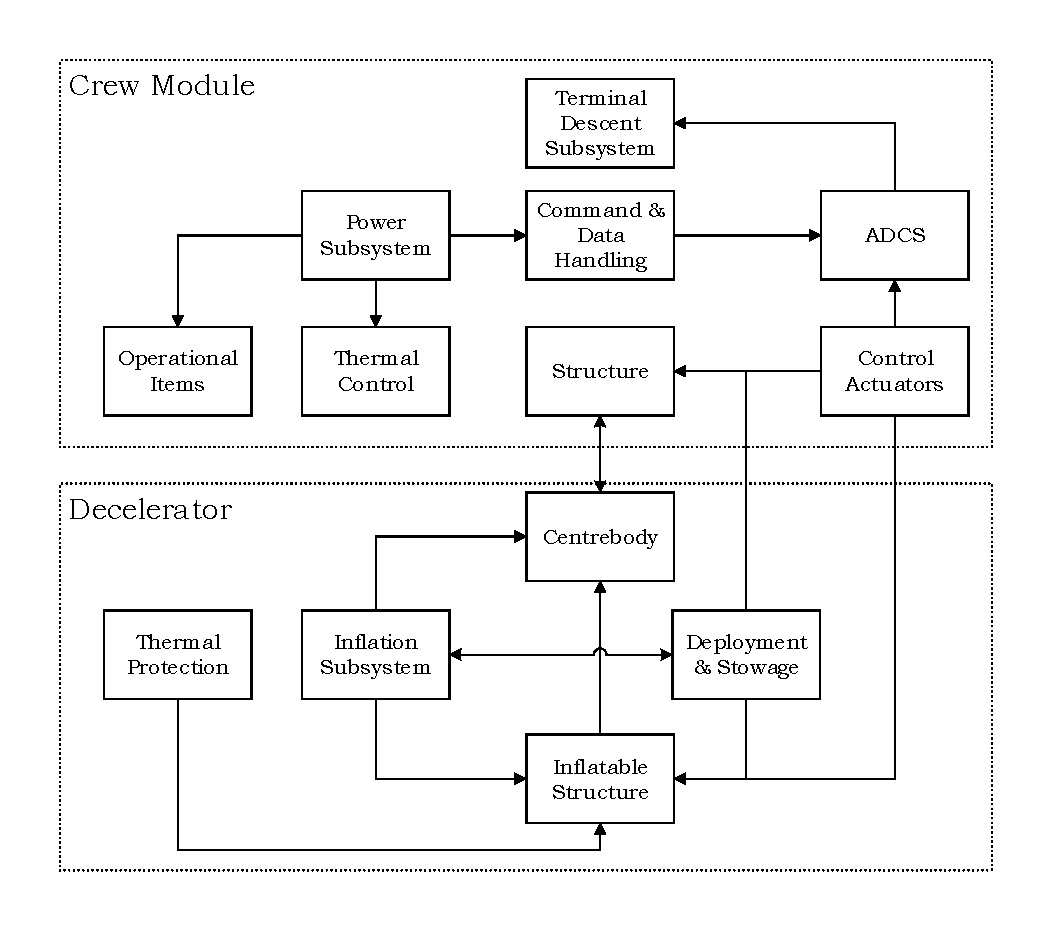
\includegraphics[width=0.95\textwidth]{./Figure/subsystem_breakdown/hardware_structure.pdf}
	\caption{Hardware diagram depicting the primary connections between the subsystems}
	\label{fig:subsystems} 
\end{figure}
%There exist some links between several of the subsystems. The \gls{tps} needs to protect the inflatable structure, centerbody, actuators and crew module. 
%
%** relation tussen inflation system, deployment en inflatable structure **
%
%** relation tussen inflatable structure en centerbody**
%
%** relation betwussen locaties actuators \& type control system (thrusters, flaps, cg offset) **
%
%** relation between actuators \& ADCS van crew module **
%
%** relatie tussen thermal control \& operational items van crew module**
%

As can be seen from Figure \ref{fig:subsystems} connections exist between several of the subsystems, both confined to the decelerator and crew module and between them. In the decelerator the inflation, deployment and stowage systems are closely related with the inflatable structure. The former two are required in order to utilise the stowed inflatable structure to fulfill its mission. The inflation system is located in the centre body. The inflatable structure is stowed against the crew module structure.

While decelerating the \gls{tps} has to protect the inflatable structure from the intense heat produced by aerodynamic forces. %At the same time the control actuators located on the inflatable structures are working to control the attitude of the spacecraft, in conjunction with the \gls{adcs}.\\

The inflatable structure is attached to the crew module structure through the rigid centre body. Control actuators can be attached to both the inflatable and crew module structure. These actuators are managed by the \gls{adcs} which receives inputs from the \gls{cdh}.\\
The power system delivers electrical power to the aforementioned \gls{cdh}, thermal control system and the operational items. At the end of the mission the \gls{adcs} provides the attitude control required for the terminal descent system.